\documentclass[PianoDiProgetto.tex]{subfiles}

\begin{document}

\chapter{Pianificazione}

\section{Analisi}
Il periodo di analisi comincia il 23-11-2017 e si conclude il 16-01-2018: l'inizio coincide con la formazione del gruppo e l'avviamento del lavoro; la conclusione con la scadenza scelta per la consegna dei documenti per l'entrata nel progetto. Durante questo periodo le attività principali svolte sono:
\begin{itemize}
	\item \textbf{Norme di Progetto:} questa attività consiste nella redazione delle \normediprogetto, un documento redatto dall'Amministratore in cui sono elencate e stabilite tutte le norme a cui il gruppo 353 deve sottostare durante tutta la durata del progetto.\\ 
	Questa attività è considerata critica dato che le \normediprogetto\ sono essenziali, infatti esse stabiliscono anche le norme e gli strumenti che verranno usati per la stesura dei documenti stessi;
	\item \textbf{Studio di Fattibilità:} questa attività consiste nella redazione da parte degli Analisti dello \studiodifattibilita, documento che contiene un'analisi dei vari capitolati proposti ed è essenziale per la scelta del capitolato che verrà svolto. \\
	L'attività è considerata critica ed è bloccante per l'inizio dell'\analisideirequisiti;
	\item \textbf{Piano di Progetto:} questa attività consiste nella redazione del \pianodiprogetto, documento nel quale il Responsabile analizza le attività necessarie e le loro scadenze per la buona riuscita del progetto. Inoltre durante questa attività vengono suddivise le risorse disponibili. L'attività è considerata critica e bloccante per la stesura della \lettera;
	\item \textbf{Piano di Qualifica}: questa attività consiste nella redazione da parte degli Analisti del \pianodiqualifica, dove si individuano i metodi per garantire la qualità del prodotto;
	\item \textbf{Glossario:} questa attività consiste nella redazione del \glossario, dove verranno inseriti tutti i termini considerati possibilmente ambigui;
	\item \textbf{Lettera di presentazione:} questa attività consiste nella redazione della \textit{Lettera di Presentazione} necessaria per la presentazione del gruppo 353 come fornitore. 	
\end{itemize}	
\begin{landscape}
	\subsection{Analisi - Diagramma di Gantt}
	\begin{figure}[ht]	
		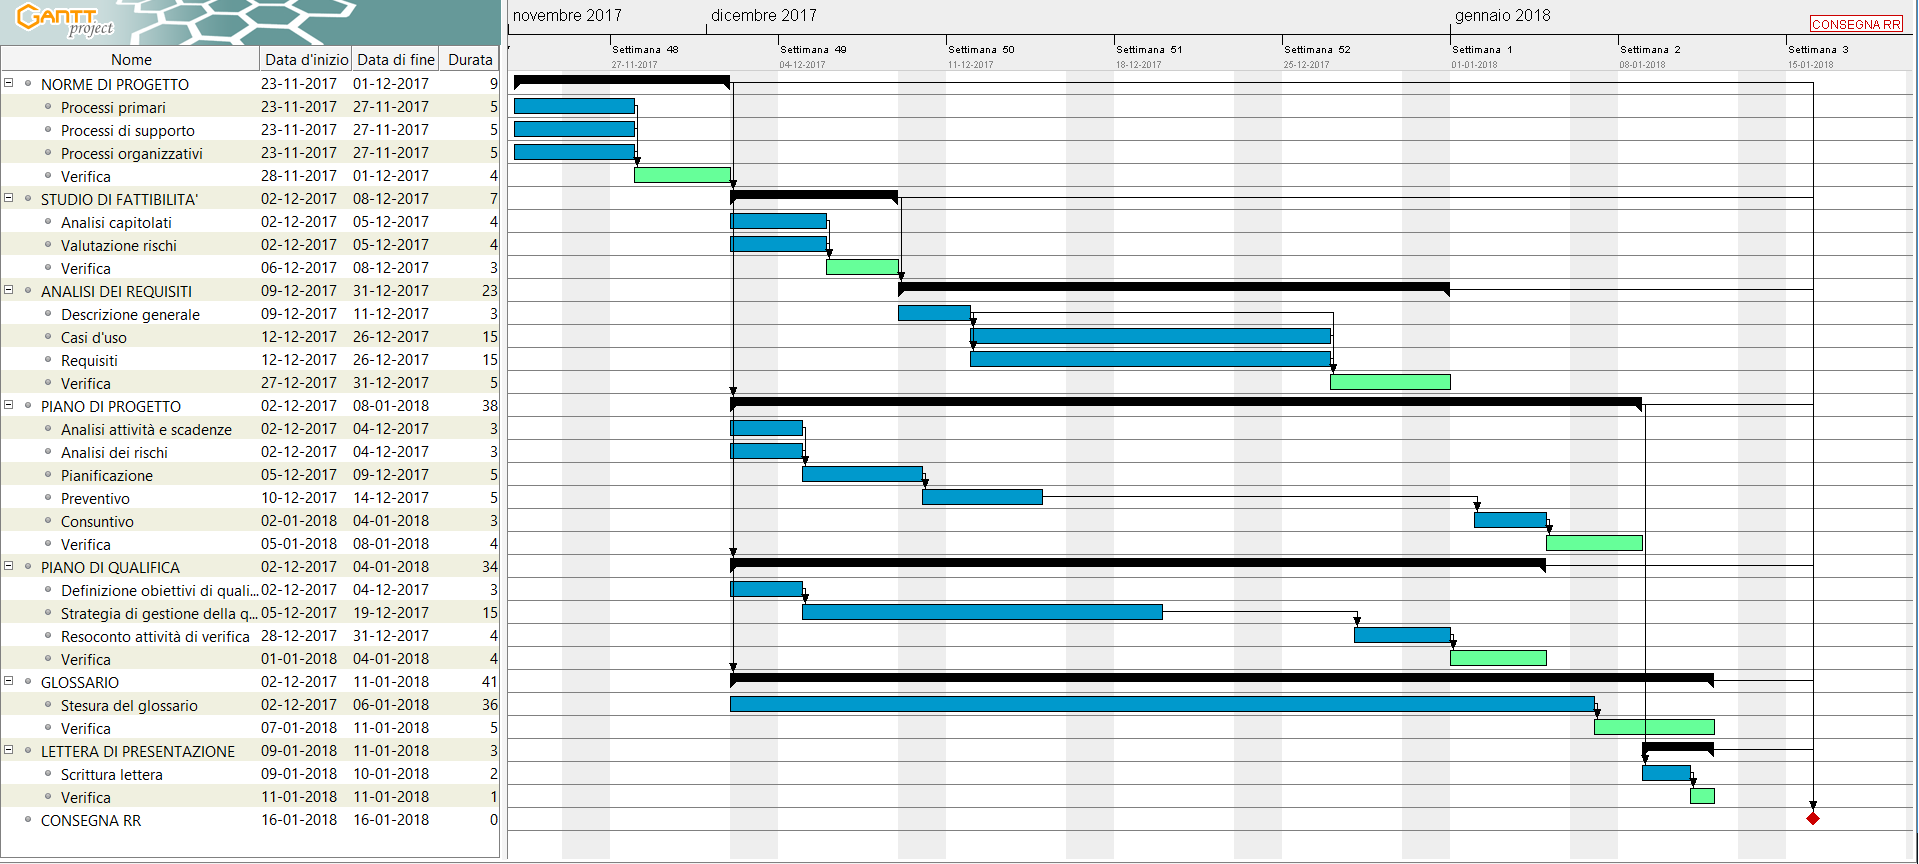
\includegraphics[width=20.5cm]{images/gantt/analisi.png}
		\label{fig:foo}
		\caption{Diagramma di Gantt del periodo di Analisi}		
	\end{figure}			
\end{landscape}	

\section{Consolidamento dei requisiti}
Il periodo di consolidamento dei requisiti inizia il 16-01-2017 e termina il 26-01-2017: comincia il giorno della consegna dei documenti per la prima scadenza e termina il giorno della presentazione della Revisione dei Requisiti. In questo periodo l'attività principale è il miglioramento dei documenti e dell'\analisideirequisiti\ in vista dell'inizio del periodo di Progettazione architetturale.
\subsection{Consolidamento dei requisiti - Diagramma di Gantt}
\begin{figure}[ht]
	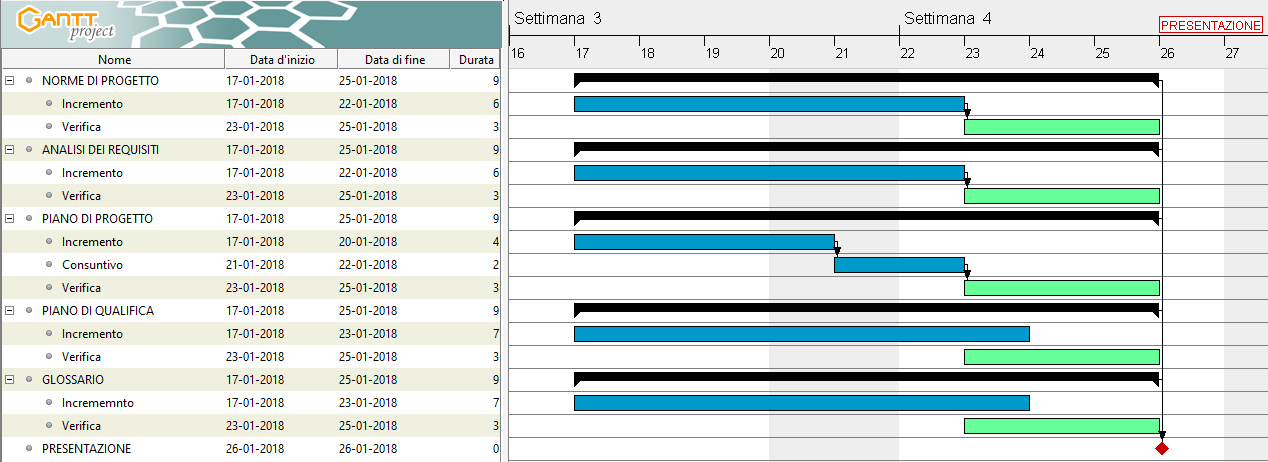
\includegraphics[width=14.5cm]{images/gantt/consolidamento.png}
	\label{fig:foo}
	\caption{Diagramma di Gantt del periodo di Consolidamento dei requisiti}
\end{figure}		


\section{Progettazione architetturale}
Il periodo di Progettazione architetturale inizia il 26-01-2017 e termina il 27-02-2017: comincia il giorno dopo la presentazione per la Revisione dei Requisiti e si conclude con la consegna dei documenti per la Revisione di Progettazione. In questo periodo, le attività principali sono:
\begin{itemize}
	\item \textbf{Incremento e Verifica:} all'inizio del periodo vengono svolte attività di Incremento e Verifica su vari documenti (\normediprogetto, \pianodiprogetto, \pianodiqualifica\ e \analisideirequisiti) e dopo la discussione Agile per il documento \technology verrà svolta anche per quest'ultimo;
	\item \textbf{Glossario:} questa attività comprende sia il miglioramento del \glossario\ che l'aggiunta di nuovi termini;
	\item \textbf{Lettera di presentazione:} questa attività prevede la stesura della \lettera per la Revisione di Progettazione;
	\item \textbf{Technology Baseline:} questa attività prevede la stesura da parte dei Progettisti del documento \technology, contenete le scelte delle tecnologie, dei framework e delle librerie per lo sviluppo del prodotto e il Proof of Concept. Questa attività è considerata critica e bloccante per la prosecuzione del progetto. In una data ancora indefinita tra il 27-02-2017 e il 12-03-2017 avvererà una discussione in modalità Agile per la verifica di questo documento.
\end{itemize}

\begin{landscape}
	\subsection{Progettazione architetturale - Diagramma di Gantt}
	\begin{figure}[ht]
		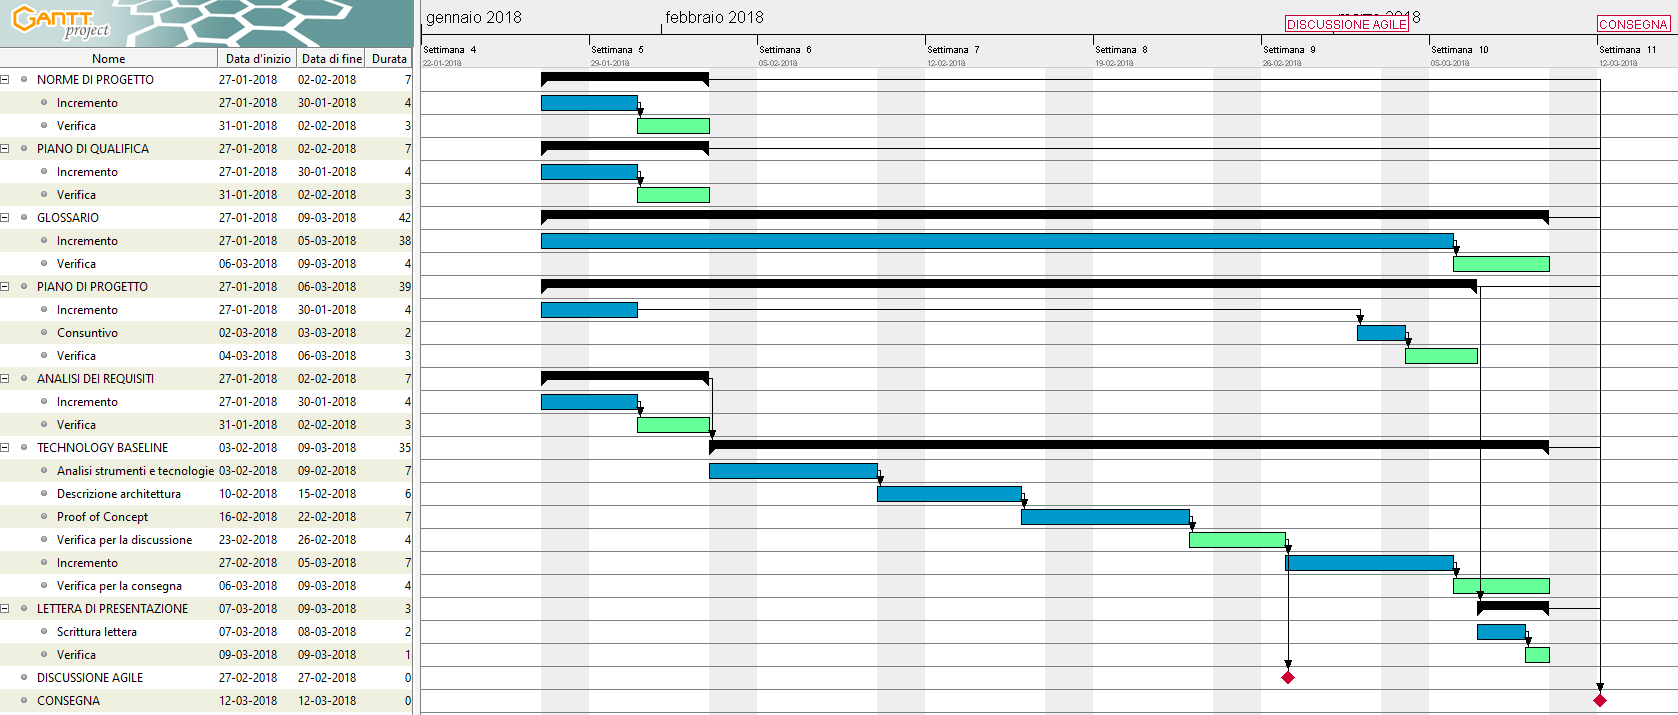
\includegraphics[width=19cm]{images/gantt/progArch.png}
		\label{fig:foo}
		\caption{Diagramma di Gantt del periodo di Progettazione architetturale}
	\end{figure}	
\end{landscape}

\section{Progettazione di dettaglio e codifica}
Il periodo di Progettazione di dettaglio e codifica inizia il 19-03-2018 e
termina il 16-04-2017: comincia il giorno stesso della Revisione di Progettazione e si conclude con la consegna dei documenti per la Revisione di
Qualifica. Durante questo periodo le attività principali svolte sono:


\begin{itemize}
	\item \textbf{Incremento e Verifica:} all'inizio del periodo vengono svolte attività di Incremento e Verifica su vari documenti (\normediprogetto, \pianodiprogetto, \pianodiqualifica\ e \technology);
	\item \textbf{Glossario:} questa attività comprende sia il miglioramento del \glossario\ che l'aggiunta di nuovi termini;
	\item \textbf{Lettera di presentazione:} questa attività prevede la stesura della lettera di presentazione per la Revisione di Qualifica;
	\item \textbf{Product Baseline:} questa attività presenta la \textit{baseline} architetturale del prodotto tramite i  diagrammi delle classi e di sequenza,
	mostrandone la coerenza con quanto mostrato durante l'attività di Technology Baseline. 
	\item \textbf{Codifica:} questa attività consiste nella scrittura del codice e nella sua verifica;
	\item \textbf{Manuale Utente:} questa attività consiste nella redazione del Manuale Utente, contenente indicazioni sull’utilizzo dell'applicazione che sta venendo prodotta.
\end{itemize}

\begin{landscape}
	\subsection{Progettazione architetturale - Diagramma di Gantt}
	\begin{figure}[ht]
		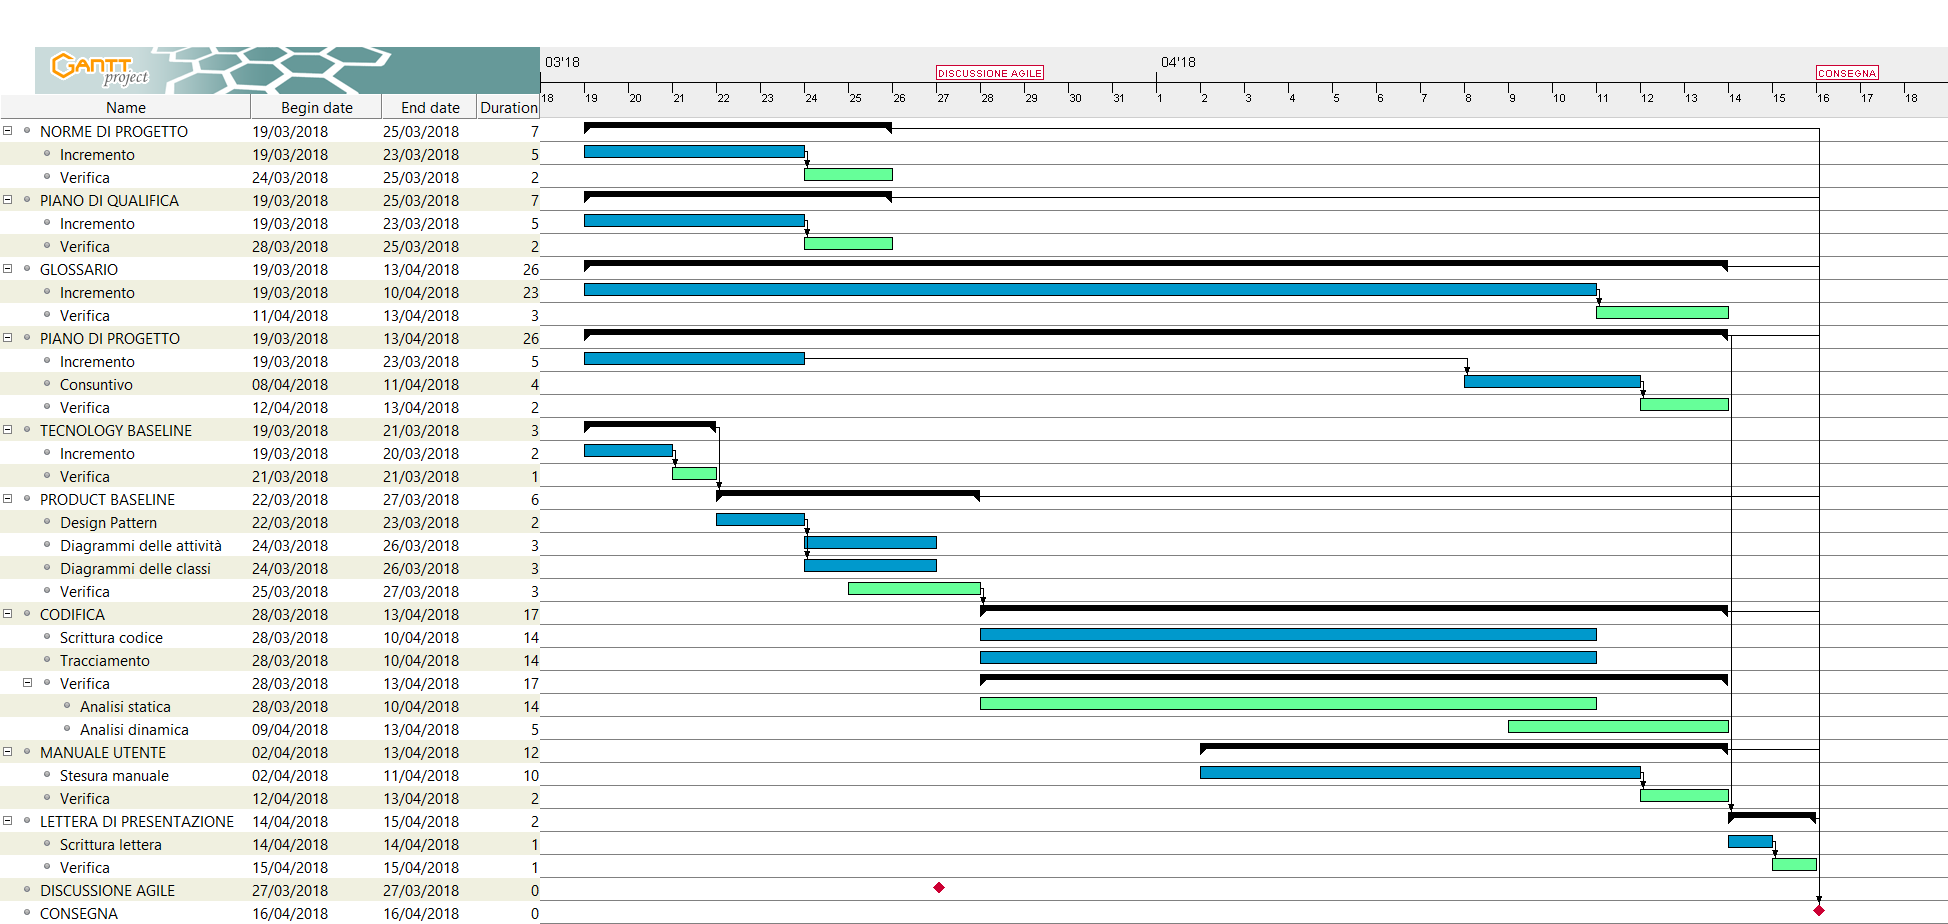
\includegraphics[width=21cm]{images/gantt/qualifica.png}
		\label{fig:foo}
		\caption{Diagramma di Gantt del periodo Progettazione di dettaglio e
			codifica}
	\end{figure}	
\end{landscape}

\section{Validazione e collaudo}
Il periodo di Validazione e collaudo inizia con il 23-04-2018 e termina il 07-05-2018: comincia il giorno stesso della Revisione di Qualifica e si conclude
con la consegna dei documenti per la Revisione di Accettazione. Durante questo periodo le attività principali svolte sono:
\begin{itemize}
\item \textbf{Incremento e Verifica:} all’inizio del periodo vengono svolte attività di Incremento e Verifica su vari documenti (\normediprogetto,\pianodiprogetto, \pianodiqualifica e \product) seguendo le indicazioni risultanti dalla Revisione di Qualifica;
\item \textbf{Glossario:} questa attività comprende sia il miglioramento del \glossario\ che l’aggiunta dei nuovi termini;
\item \textbf{Validazione e Collaudo:} questa attività consiste nell’esecuzione di ulteriori test e miglioramenti dell'applicazione prodotto per assicurare che soddisfi tutti i vincoli qualitativi;
\item  \textbf{Manuale Utente:} questa attività consiste nel miglioramento e completamento del \manualeutente, contenente indicazioni sull’utilizzo dell'applicazione.
\end{itemize}
\begin{landscape}
\subsection{Validazione e collaudo - Diagramma di Gantt}
\begin{figure}[ht]
	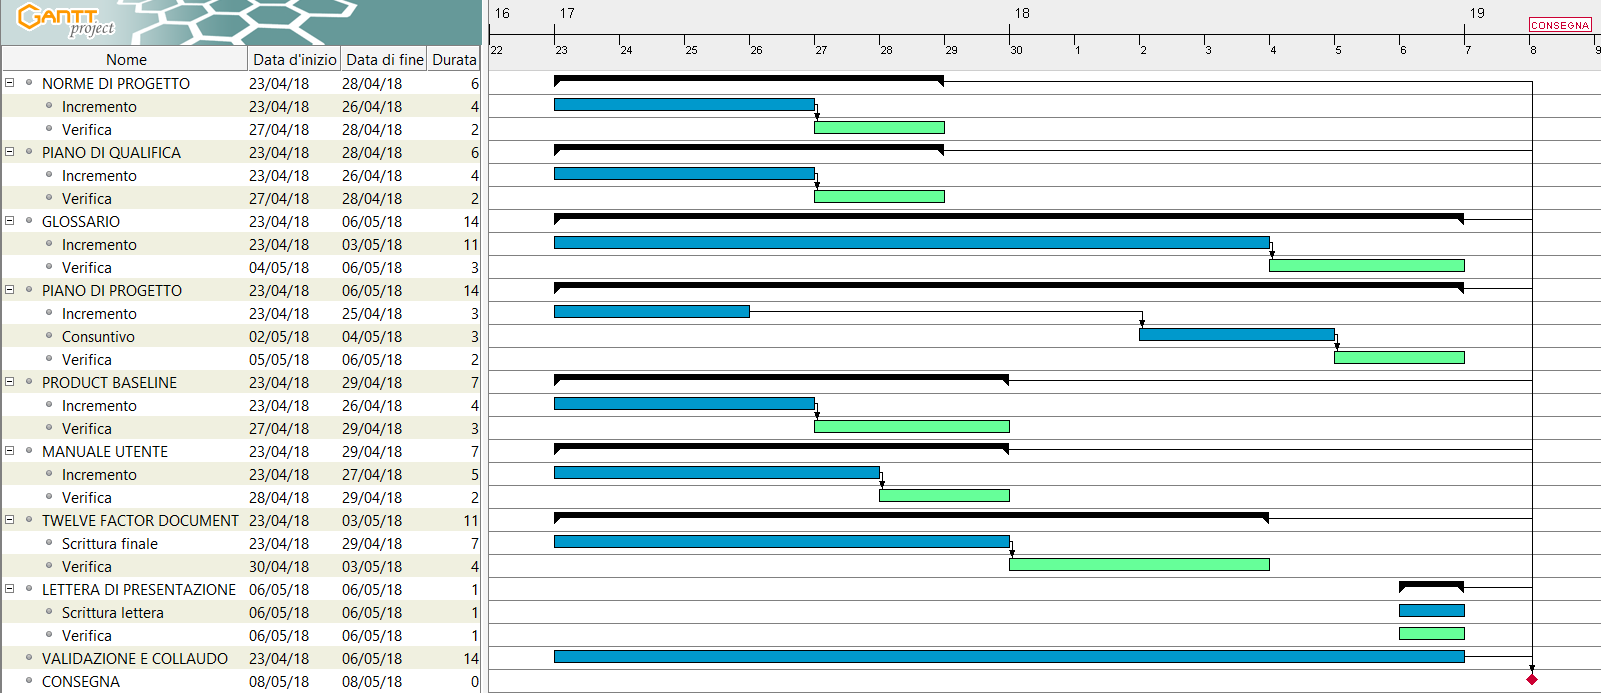
\includegraphics[width=21cm]{images/gantt/collaudo.png}
	\label{fig:foo}
	\caption{Diagramma di Gantt del periodo Validazione e collaudo}
\end{figure}
\end{landscape}	
\end{document}